\section{Netwerkeigenschappen}\label{sec:tests} \label{sec:tests}
In dit hoofdstuk zal er gekeken worden naar een aantal eigenschappen van het netwerk. Er zal onder andere gekeken worden naar het effect van het zendvermogen op de betrouwbaarheid van bericht aankomst.

\subsection{Invloed van afstand tussen twee nodes} \label{sec:influenceOfDistanceOnNetwork}
De afstand tussen twee netwerk nodes heeft invloed op de betrouwbaarheid van het netwerk. Er moet dus onderzocht worden wat de invloed van afstand tussen netwerk nodes is op het netwerk. Omdat het zendvermogen erg veel invloed heeft op over welke afstand er informatie kan worden overgedragen, zal het zendvermogen ook worden meegenomen.

\begin{figure}[h]
    \centering
    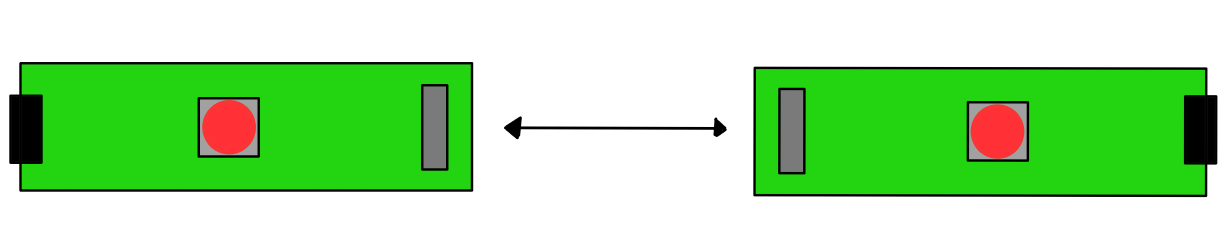
\includegraphics[scale = 0.3]{img/test1.png}
    \caption{Test opstelling.}
    \label{fig:TestCom}
\end{figure}
Om de invloed van afstand tussen twee netwerk nodes te onderzoeken, zal gebruik gemaakt worden van de test opstelling die schematisch is weergegeven in \autoref{fig:TestCom}. Er zal met verschillende afstanden tussen de twee netwerk nodes gemeten hoeveel procent er van de verstuurde berichten aankomen. Deze metingen zullen gedaan worden op twee zendvermogens, -12dBm en -18dBm respectievelijk.

\begin{figure}[ht]
    \centering
    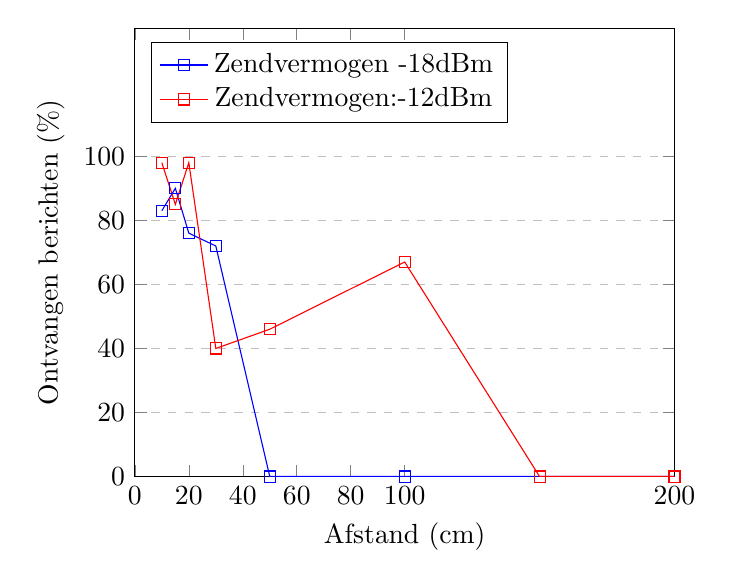
\begin{tikzpicture}
    \begin{axis}[
        xlabel={Afstand (cm)},
        ylabel={Ontvangen berichten (\%)},
        xmin=0, xmax=200,
        ymin=0, ymax=140,
        xtick={0,20,40,60,80,100,200},
        ytick={0,20,40,60,80,100},
        legend pos=north west,
        ymajorgrids=true,
        grid style=dashed,
    ]

    \addplot[
        color=blue,
        mark=square,
        ]
        coordinates {
        (10,83)(15,90)(20,76)(30,72)(50,0)(100,0)(150,0)(200,0)
        };
        \addlegendentry{Zendvermogen -18dBm}

    \addplot[
        color=red,
        mark=square,
        ]
        coordinates {
        (10,98)(15,85)(20,98)(30,40)(50,46)(100,67)(150,0)(200,0)
        };
        \addlegendentry{Zendvermogen:-12dBm}
        
    \end{axis}
    \end{tikzpicture}
    \caption{Resultaten van de metingen die gedaan zijn met de testopstelling van \autoref{fig:TestCom}.}
    \label{fig:resultsOfDistanceMeasurements}
\end{figure}
De data die is verzameld met het uitvoeren van de metingen, zoals eerder beschreven in deze paragraaf worden getoond in \autoref{fig:resultsOfDistanceMeasurements}. Het is erg belangrijk om te vermelden dat al deze metingen eenmalig zijn uitgevoerd.

\subsection{Hop Test} \label{sec:influenceOfHopsInNetwork}
Met deze test wordt er gekeken naar de invloed op de ontvangstkans als er niet een directe verbinding is tussen twee nodes. Om dit te onderzoeken zal gebruik gemaakt worden van de testopstelling die schematisch is weergegeven in \autoref{fig:Testhop}. 
\begin{figure}[h]
    \centering
    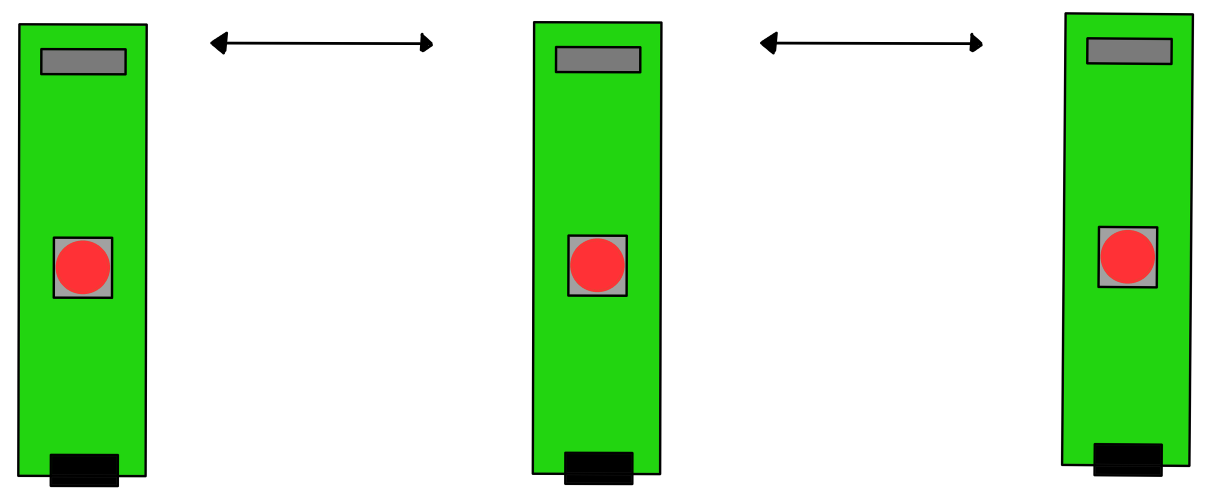
\includegraphics[scale = 0.4]{img/test2.png}
    \caption{Test opstelling 2}
    \label{fig:Testhop}
\end{figure}
De afstand tussen node één en node twee zijn gelijk aan de afstand tussen node twee en drie. Node één zal 100 berichten via node 2 naar node drie sturen. Er wordt bijgehouden hoeveel van deze berichten aankomen. Het aantal berichten dat aankomt is een indicatie voor de invloed van het sturen van data via andere nodes in het netwerk.

Uit de test is gebleken dat de betrouwbaarheid van bericht aankomst 81\% is. Het is belangrijk om te vermelden dat dit resultaat op een enkele meeting is gebaseerd.

\subsection{Conclusies op basis de metingen}
In paragrafen \ref{sec:influenceOfDistanceOnNetwork} en \ref{sec:influenceOfHopsInNetwork} zijn een aantal metingen gedaan aan het netwerk. Uit deze metingen valt te halen dat er niet een vergrote kans is op het niet aankomen van berichten, op het moment dat deze via een andere node worden verstuurd. Wel is aangetoond dat de afstand tussen twee netwerk nodes een zeer bepalende factor heeft op de kans of berichten aankomen.